\documentclass[aspectratio=169,11pt]{beamer}
\makeatletter
\input{../../templates/dune-professional/beamerthemeDUNEProfessional.sty}
\makeatother
\usepackage{fancyvrb}
\title{Slow-controls simulation}
\subtitle{Updated VD and HD results; a short guide to running them}
\author{Manuel Arroyave}
\date{6 October 2026}
\newcommand{\mydate}{6 October 2026}
\hypersetup{colorlinks=true,urlcolor=DuneInfo,linkcolor=DuneInfo}
\newcommand{\Source}[1]{\par\smallskip{\footnotesize\color{DuneTextMuted}#1\par}}
\newcommand{\Command}[1]{\VerbatimInput[fontsize=\small]{commands/#1}}

\begin{document}
\begin{frame}[plain]
  \titlepage
\end{frame}

\begin{frame}{Monitoring: two processes per detector}
  \DuneBigStatement{VD AND HD TESTED SEPARATELY}
    {Two processes reached 95\% of the best throughput}
    {All 12 process-count checks passed, with zero read errors.}
  \medskip
  \centering
  \begin{tabular}{lrrrr}
    \toprule
    Detector & WIBs & DAPHNEs & Read values/s & Memory \\
    \midrule
    VD & 480 & 42 & 131,838 & 296 MB \\
    HD & 750 & 150 & 129,467 & 354 MB \\
    \bottomrule
  \end{tabular}
  \Source{[L1] At two OPC-UA processes on one test host. Board-only model: 17 variables/WIB, 21/DAPHNE; PTCs and other systems excluded.}
\end{frame}

\begin{frame}{Beyond two processes, throughput changes little}
  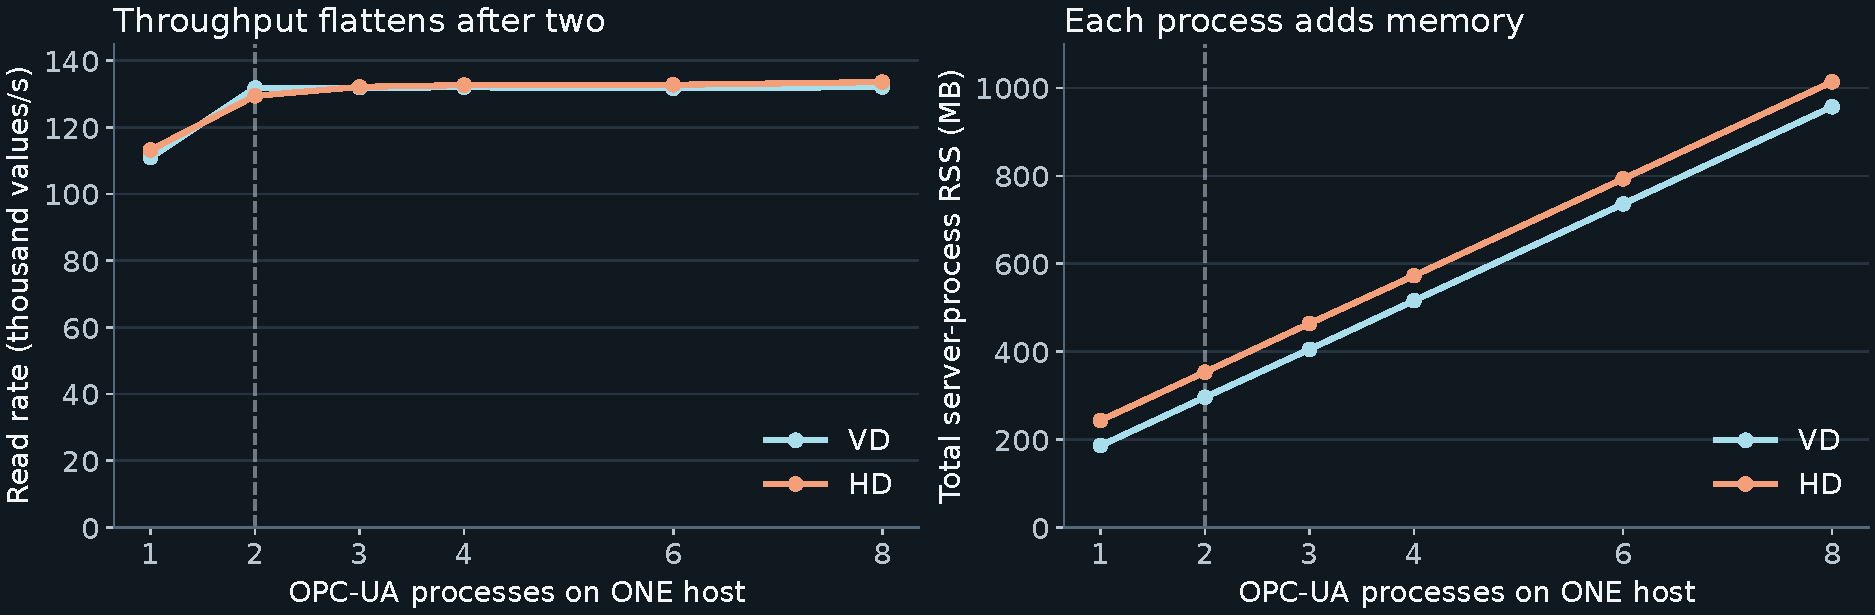
\includegraphics[width=\textwidth]{figures/process-curve.pdf}
  \DuneDiagramCaption{Sweep: 1, 2, 3, 4, 6 and 8 OPC-UA programs sharing one test host.}
  \Source{[L1] One representative value/board changes every 250 ms. VD DAPHNE interference fell from +13.1\% at two processes to +1.3\% at four.}
\end{frame}

\begin{frame}{Configuring and checking one WIB is one job}
  \DuneCompactColorBlock{coral}{QUEUE MODEL}{48 simultaneous WIB jobs per bridge}
    {Each worker configures one board, reads its settings back, then takes the next board.}
  \medskip
  \centering
  \begin{tabular}{lrrrrr}
    \toprule
    Detector & Bridges & WIBs/bridge & Batches & p95 & p99 \\
    \midrule
    VD & 4 & 120 & 3 & \textbf{48.42 s} & 78.41 s \\
    HD & 6 & 125 & 3 & \textbf{62.28 s} & 78.41 s \\
    HD comparison & 4 & 187--188 & 4 & 78.41 s & 94.55 s \\
    \bottomrule
  \end{tabular}
  \Source{[Q1] VD batches: 48 + 48 + 24; HD/six bridges: 48 + 48 + 29. Assumes 16.10 s/WIB, network delays and retries; HD reuses VD timings. Projections, not measured hardware completion.}
\end{frame}

\begin{frame}{Physical servers: test one host per detector}
  \begin{columns}[T,onlytextwidth]
    \begin{column}{0.48\textwidth}
      \DuneFixedColorBlock{sky}{2.8cm}{BRIDGE-HOST PROPOSAL}{2 active hosts total}
        {One for VD, one for HD.\par\medskip Dedicated failover partners would make four.}
    \end{column}
    \begin{column}{0.48\textwidth}
      \DuneFixedColorBlock{paper}{2.8cm}{STILL TO VALIDATE}{Full production load}
        {PTCs, other interfaces, full namespaces, native latency, Ignition/historian load and failover.}
    \end{column}
  \end{columns}
  \Source{[L1] A production minimum is unmeasured. The populations ran separately on one test host. Ignition, database and instrument PCs require separate sizing.}
\end{frame}

\begin{frame}[fragile]{Run it: open a terminal in your sc\_emu checkout}
  \Command{setup-smoke.sh}
  \bigskip
  \DuneCompactColorBlock{paper}{REQUIREMENTS}{Linux/WSL, Python 3.13, internet for setup}
    {Use the updated checkout containing \texttt{tools/setup.sh}. The installation creates \texttt{.venv} in that checkout.}
  \smallskip
  \DuneCompactColorBlock{sky}{SMALL CHECK}{Wait for PASS: 2 topologies completed}
    {Uses 6 WIBs + 2 DAPHNEs; no detector hardware needed.}
  \Source{[R1] Run all following commands from this repository directory, wherever you keep it.}
\end{frame}

\begin{frame}[fragile]{Run VD, then HD, then open the reports}
  \Command{updated-runs.sh}
  \bigskip
  \DuneCompactColorBlock{sky}{EACH RUN}{Wait for PASS: 6 topologies completed}
    {Allow several minutes. In the report viewer, use arrow keys to scroll and q to quit.}
  \Source{[R1] Keep the timestamped run directory: report, inventory, provenance and package versions. Timings vary by computer.}
\end{frame}

\begin{frame}[fragile]{Optional: rerun the configuration projection}
  \Command{queues.sh}
  \medskip
  \DuneCompactColorBlock{sky}{OUTPUT}{Open report.md in the printed run directory}
    {Run after VD and HD finish. Full instructions: \texttt{sc\_emu/RUNBOOK.md}.}
  \medskip
  \begin{tabular}{lp{8.6cm}}
    \toprule
    Report term & Meaning \\
    \midrule
    Values/s & Completed OPC-UA Read values per second \\
    RSS & Server-process memory \\
    p95 & 95\% of observed or modeled times are at or below this value \\
    \bottomrule
  \end{tabular}
  \Source{[Q1, R1] Raw reports and simulation code belong to sc\_emu. Source links and assumptions: SOURCES.md.}
\end{frame}
\end{document}
